\documentclass[../MA_Thesis.tex]{subfiles}
\renewcommand{\baselinestretch}{1.5} 
\usepackage{hyperref}
\usepackage{csquotes}

% Configuration for the listings package
\lstset{
    frame=single, % Add a frame around the code
    basicstyle=\ttfamily\footnotesize, % Set the basic font style and size
    keywordstyle=\color{blue}, % Set the color for keywords
    commentstyle=\color{green}, % Set the color for comments
    stringstyle=\color{red}, % Set the color for strings
    numbers=left, % Show line numbers on the left
    numberstyle=\tiny\color{gray}, % Style for line numbers
    stepnumber=1, % Show every line number
    numbersep=5pt, % Distance from the code to the line numbers
    backgroundcolor=\color{white}, % Background color for the code
    showspaces=false, % Show spaces as visible characters
    showstringspaces=false, % Show spaces in strings as visible characters
    breaklines=true, % Automatically break long lines
    captionpos=b, % Set the caption position to bottom
    language=Python % Set the default language
}

\begin{document}
\begin{appendix}
\section{Sample Completed Drawings}
\label{appendix: sample_completed_drawings}

This section presents sample completed drawings from three different stimulus groups (A, B, and C) in the Incomplete Shape Drawing Task.

\begin{figure}[H]
\centering
\textbf{Sample Completions from Group A Stimuli}\par\medskip
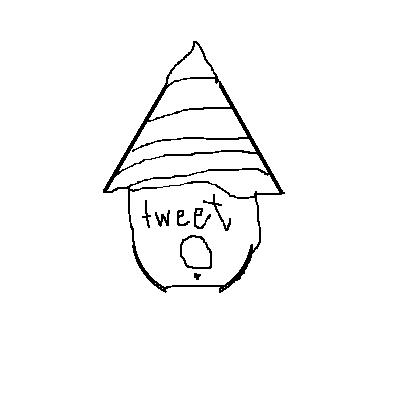
\includegraphics[width=0.3\textwidth]{sample_completed_shapes/Group_1_Sample_1.png}
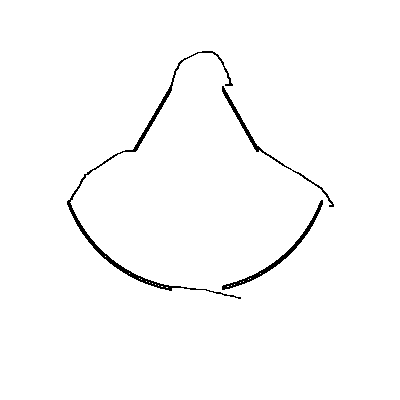
\includegraphics[width=0.3\textwidth]{sample_completed_shapes/Group_1_Sample_2.png}

\includegraphics[width=0.3\textwidth]{sample_completed_shapes/Group_1_Sample_3.png}
\end{figure}

\begin{figure}[H]
\centering
\textbf{Sample Completions from Group B Stimuli}\par\medskip
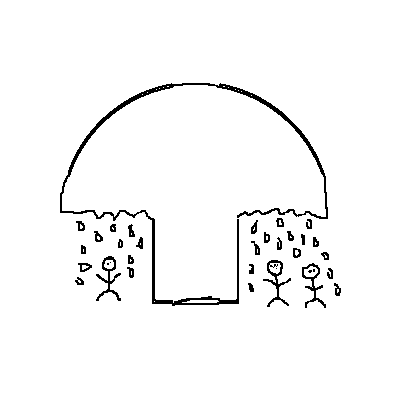
\includegraphics[width=0.3\textwidth]{sample_completed_shapes/Group_2_Sample_1.png}
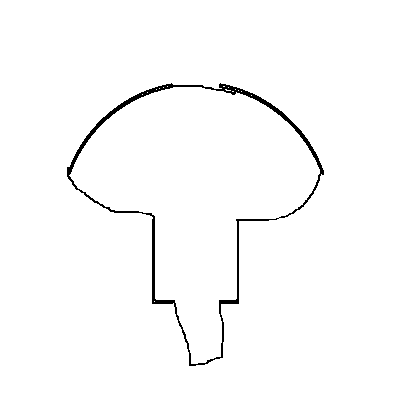
\includegraphics[width=0.3\textwidth]{sample_completed_shapes/Group_2_Sample_2.png}
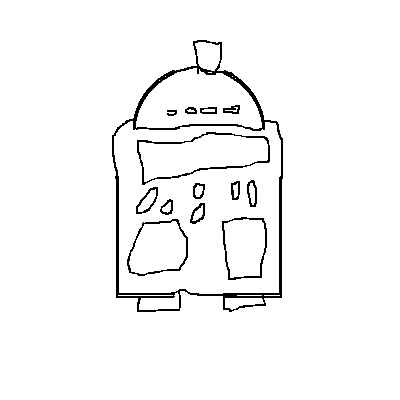
\includegraphics[width=0.3\textwidth]{sample_completed_shapes/Group_2_Sample_3.png}
\end{figure}

\begin{figure}[H]
\centering
\textbf{Sample Completions from Group C Stimuli}\par\medskip
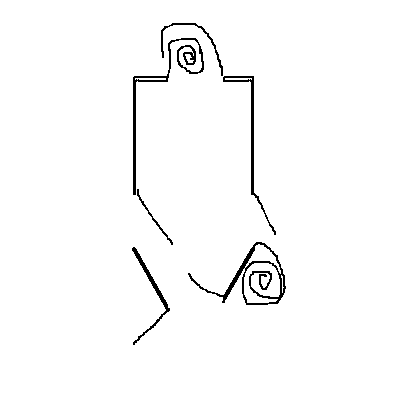
\includegraphics[width=0.3\textwidth]{sample_completed_shapes/Group_3_Sample_1.png}
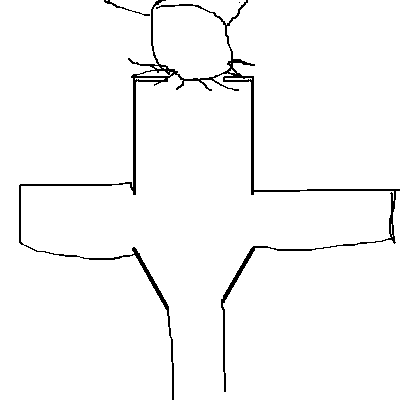
\includegraphics[width=0.3\textwidth]{sample_completed_shapes/Group_3_Sample_2.png}
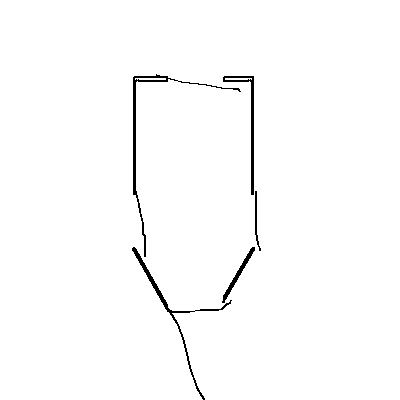
\includegraphics[width=0.3\textwidth]{sample_completed_shapes/Group_3_Sample_3.png}
\end{figure}

% Formula for Entropy of the Gaussian Mixture Model
\newpage
\section{Formula for Calculating Entropy of the Gaussian Mixture Model}
\label{appendix: entropy}
This study adopts the approach proposed by \textcite{huber_entropy_2008} to approximate the entropy of a GMM by incorporating the Kullback-Leibler (KL) divergence between each pair of components within the mixture, as suggested by \textcite{hershey_approximating_2007}:
\begin{equation*}
    H(GMM) \approx -\sum_{i=1}^{N} \pi_i \log \left(\sum_{j=1}^{N} \pi_j \exp\left(-\frac{1}{2} D_{KL}(N_i || N_j)\right)\right),
\end{equation*}
\begin{equation*}
    D_{KL}(N_i || N_j) = \frac{1}{2} \left( \text{tr}(\Sigma_j^{-1}\Sigma_i) + (\mu_j - \mu_i)^T \Sigma_j^{-1} (\mu_j - \mu_i) - k + \ln\left(\frac{|\Sigma_j|}{|\Sigma_i|}\right) \right),
\end{equation*}
where:
\begin{itemize}
    \item \(N\) represents the number of components in the GMM.
    \item \(\pi_i\) and \(\pi_j\) are the mixing coefficients for components \(i\) and \(j\), respectively, indicating the weight of each component in the mixture.
    \item \(D_{KL}(N_i || N_j)\) measures the divergence between the \(i\)-th and \(j\)-th components of the GMM, quantifying the difference between these two probability distributions.
    \item \(\Sigma_i\) and \(\Sigma_j\) are the covariance matrices of components \(N_i\) and \(N_j\), respectively.
    \item \(\mu_i\) and \(\mu_j\) are the mean vectors of components \(N_i\) and \(N_j\), respectively.
    \item \(\text{tr}(\cdot)\) denotes the trace of a matrix, the sum of its diagonal elements.
    \item \(k\) is the dimensionality of the data or the number of features in the dataset.
    \item \(|\Sigma|\) denotes the determinant of the covariance matrix \(\Sigma\).
\end{itemize}

% Formula for Aggregated Bhattacharyya Distance
\newpage
\section{Formula for Calculating Aggregated Bhattacharyya Distance}
\label{appendix: bhattacharyya distance}
Given a Gaussian Mixture Model (GMM) with $N$ components, each defined by a mean vector $\mu_i$ and a covariance matrix $\Sigma_i$, the Bhattacharyya distance ($D_B$) between any two components $i$ and $j$ can be calculated as:
    \begin{equation*}
        BC[\mu_i, \Sigma_i, \mu_j, \Sigma_j] = \left| \frac{\Sigma_i + \Sigma_j}{2} \right|^{-\frac{1}{2}} \cdot \left|\Sigma_i\right|^\frac{1}{4} \cdot \left|\Sigma_j\right|^\frac{1}{4} \cdot \exp\left( -\frac{1}{8} \Delta\mu_{ij}^T \left(\frac{\Sigma_i + \Sigma_j}{2}\right)^{-1} \Delta\mu_{ij} \right)
    \end{equation*}
    where $\Delta\mu_{ij} = \mu_j - \mu_i$ is the difference between the mean vectors of components $i$ and $j$. To compute the aggregated Bhattacharyya distance ($D_{AB}$) across all unique pairs of components in the GMM, one option would be averaging the distances calculated using the formula above:
    \begin{equation*}
        D_{AB} = \frac{1}{\binom{2}{N}} \sum_{i=1}^{N-1} \sum_{j=i+1}^{N} BC[\mu_i, \Sigma_i, \mu_j, \Sigma_j].
    \end{equation*}

% Formula for DSI
\newpage
\section{Formula for Calculating Divergent Semantic Integration}
\label{appendix: DSI}
After converting narrative texts into BERT word embeddings, pairwise semantic distances are calculated, which are further used to derive DSI scores using the following formula (\cite{johnson_divergent_2022}):
\begin{equation*}
    DSI = \frac{2}{n(n-1)} \sum_{i=1}^{n} \sum_{k=i+1}^{n} D_{\text{cos}}(\omega_i, \omega_k)
\end{equation*}
\begin{equation*}
    D_{\text{cos}}(\omega, k) = 1 - \frac{\omega \cdot k}{\|\omega\| \|k\|}
\end{equation*}
where:
\begin{itemize}
    \item \(\omega_i, \omega_k\) are the embeddings for words \(i\) and \(k\).
    \item \(D_{\text{cos}}\) measures the cosine distance, which is 1 minus the cosine similarity, between the embeddings.
    \item \(n\) is the number of unique word pairs considered.
\end{itemize}

% (Insignificant) Mediation Results
\newpage
\section{Mediation Analysis}
\label{appendix: mediation_analysis_results}
To evaluate whether mood condition influenced creative originality through different aspects of cognitive flexibility, a series of mediation models were conducted, testing each flexibility measure individually as a mediator. Mood conditions were dummy-coded using the Neutral Control group as the reference category. The outcome variable in all models was originality, measured via AuDrA (see Table~\ref{tab:mediation_summary} for detailed mediation results).

\paragraph{Average Entropy.}
Mood condition had no significant effect on average entropy (D1: $\beta = -0.010$, $p = .646$; D2: $\beta = -0.046$, $p = .039$), and average entropy did not significantly predict originality ($\beta = -0.255$, $p = .010$). While the path b effect was statistically significant, the indirect effects were not: indirect$_{D1}$ = 0.003 ($p = .672$), indirect$_{D2}$ = 0.012 ($p = .106$). Direct effects of mood on originality were non-significant, and total effects were close to zero.

\paragraph{Average Bhattacharyya Distance.}
Neither mood condition (D1: $\beta = -0.042$, $p = .552$; D2: $\beta = -0.107$, $p = .113$) nor average Bhattacharyya distance ($\beta = -0.037$, $p = .239$) significantly predicted originality. Indirect effects were also non-significant (indirect$_{D1}$ = 0.002, $p = .658$; indirect$_{D2}$ = 0.004, $p = .359$), and direct effects remained negligible.

\paragraph{Inflection Proportion of Entropy.}
Mood condition had no significant effect on inflection proportion (D1: $\beta = 0.018$, $p = .649$; D2: $\beta = 0.042$, $p = .268$), but inflection proportion strongly predicted originality ($\beta = 0.447$, $p < .001$). Indirect effects were not significant (indirect$_{D1}$ = 0.008, $p = .652$; indirect$_{D2}$ = 0.019, $p = .266$), but the strength of the b-path suggests this mediator may still play a functional role. Direct effects remained non-significant.

\paragraph{Inflection Proportion of Bhattacharyya Distance.}
Patterns were similar: no significant effect of mood condition on the mediator (D1: $\beta = 0.024$, $p = .540$; D2: $\beta = 0.027$, $p = .510$), but a strong effect of inflection proportion on originality ($\beta = 0.446$, $p < .001$). Indirect effects again were non-significant (indirect$_{D1}$ = 0.011, $p = .542$; indirect$_{D2}$ = 0.012, $p = .511$).

\paragraph{Divergent Semantic Integration (DSI).}
DSI was weakly predicted by mood condition (D1: $\beta = 0.078$, $p = .163$; D2: $\beta = 0.008$, $p = .897$), but it significantly predicted originality ($\beta = 0.219$, $p < .001$). Although the indirect effects were not statistically significant (indirect$_{D1}$ = 0.017, $p = .177$; indirect$_{D2}$ = 0.002, $p = .898$), the direct effects of mood on originality were also non-significant, suggesting a partial mediation.

Overall, while mood induction did not significantly influence most flexibility measures, originality was reliably predicted by DSI and inflection-based flexibility. These findings support the notion that originality may depend more on dynamic, adaptive shifts and conceptual integration rather than on sustained exploratory breadth alone.

\begin{table}[H]
{\fontsize{9pt}{11pt}\selectfont
\centering
\caption{Mediation Model Summary: Flexibility Measures as Mediators of Mood on Originality}
\label{tab:mediation_summary}
\begin{tabular}{lcccc}
\toprule
\textbf{Mediator} & \textbf{Path a} ($\beta$) & \textbf{Path b} ($\beta$) & \textbf{Indirect Effect} & \textbf{Direct Effect} \\
\midrule
Avg. Entropy & D1: –0.010 ($p = .646$) & –0.255*** ($p = .010$) & D1: 0.003 [–.010, .015] ($p = .672$) & D1: –0.006 ($p = .759$) \\
             & D2: –0.046* ($p = .039$) &                         & D2: 0.012 [–.000, .028] ($p = .106$) & D2: –0.005 ($p = .821$) \\
\addlinespace
Avg. Bhatt. Dist. & D1: –0.042 ($p = .552$) & –0.037 ($p = .239$) & D1: 0.002 [–.005, .009] ($p = .658$) & D1: –0.005 ($p = .803$) \\
                  & D2: –0.107 ($p = .113$) &                     & D2: 0.004 [–.003, .015] ($p = .359$) & D2:  0.003 ($p = .899$) \\
\addlinespace
Inflect. Prop. Entropy & D1:  0.018 ($p = .649$) &  0.447*** ($p < .001$) & D1: 0.008 [–.027, .043] ($p = .652$) & D1: –0.011 ($p = .326$) \\
                       & D2:  0.042 ($p = .268$) &                         & D2: 0.019 [–.015, .052] ($p = .266$) & D2: –0.012 ($p = .285$) \\
\addlinespace
Inflect. Prop. Bhatt & D1:  0.024 ($p = .540$) &  0.446*** ($p < .001$) & D1: 0.011 [–.024, .046] ($p = .542$) & D1: –0.014 ($p = .162$) \\
                     & D2:  0.027 ($p = .510$) &                        & D2: 0.012 [–.025, .047] ($p = .511$) & D2: –0.005 ($p = .609$) \\
\addlinespace
DSI & D1: 0.078 ($p = .163$) & 0.219*** ($p < .001$) & D1: 0.017 [–.006, .045] ($p = .177$) & D1: –0.021 ($p = .213$) \\
    & D2: 0.008 ($p = .897$) &                        & D2: 0.002 [–.023, .028] ($p = .898$) & D2:  0.005 ($p = .749$) \\
\bottomrule
\end{tabular}
\begin{tablenotes}[flushleft]
\small
\item \textit{Note.} * $p < .05$, ** $p < .01$, *** $p < .001$. Path a = Mood group $\rightarrow$ Flexibility; Path b = Flexibility $\rightarrow$ Originality (AuDrA); Indirect effect = $\text{a} \times \text{b}$; D1 = High Arousal vs. Neutral; D2 = Low Arousal vs. Neutral. Confidence intervals based on 5,000 bootstrapped samples.
\end{tablenotes}
}
\end{table}

\end{appendix}
\end{document}